% DOC SETTINGS ===================================
\documentclass{article}
\usepackage[utf8]{inputenc}
\usepackage{fancyhdr}
\pagestyle{fancy}
\usepackage{geometry}
 \geometry{
 a4paper,
 total={170mm,257mm},
 left=20mm,
 top=25mm,
 }
\fancyheadoffset{0mm}
\lhead{ECE3544 Lab 1.A Report}
\rhead{Kavin Thirukonda 2021}
\usepackage{steinmetz}
\usepackage{listings}
\usepackage{longtable}
\usepackage{circuitikz}
\usepackage{mathtools}  
\mathtoolsset{showonlyrefs} 
\cfoot{}
% DOC SETTINGS ===================================
\begin{document}
\begin{center}
    \vspace*{1cm}
    \Huge
    \textbf{ECE3544 Lab 1 Report}
    
    \vspace{0.5cm}
    \LARGE
    Section A
    
    \vspace{1.5cm}
    \textbf{Kavin Thirukonda}
    \vfill
    \small
    Description:
    
    This is the formal lab report for Lab 1.A to discuss the objectives, constraints, design, optimization, and implementation of Lab 1.A.
    \vspace{10cm}
\end{center}
\newpage
\section{Objectives}
The objectives of this project is to become more familiar with verilog structural code once again as well as modelsim coding and testing. That includes using the model sim program itself as well as launching waveform test benches, also making project, coding .v files, and making test benches.
\section{Block Diagram Representations}
\begin{center}
    \boxed{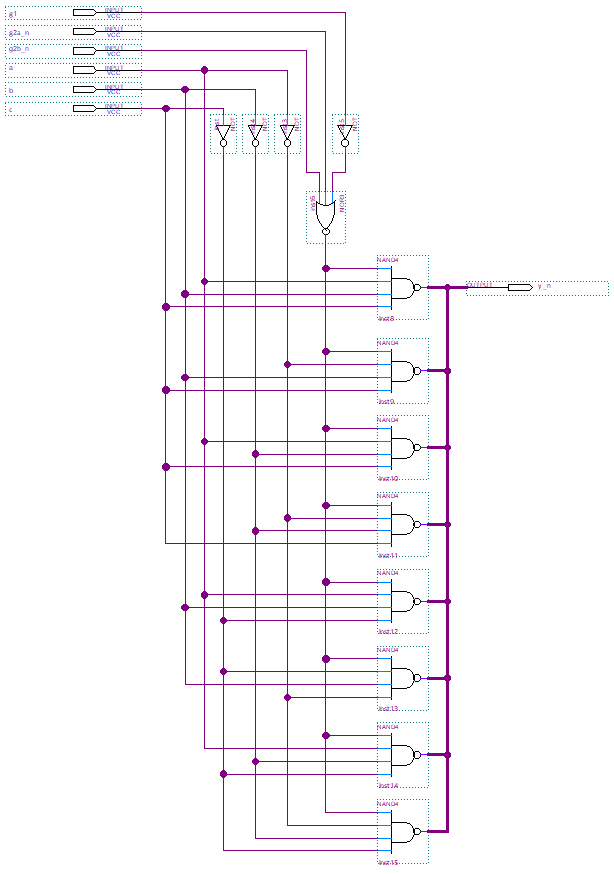
\includegraphics[angle=90,origin=c,width = .7\textwidth]{bdf1.png}}
\end{center}
\begin{center}
    \boxed{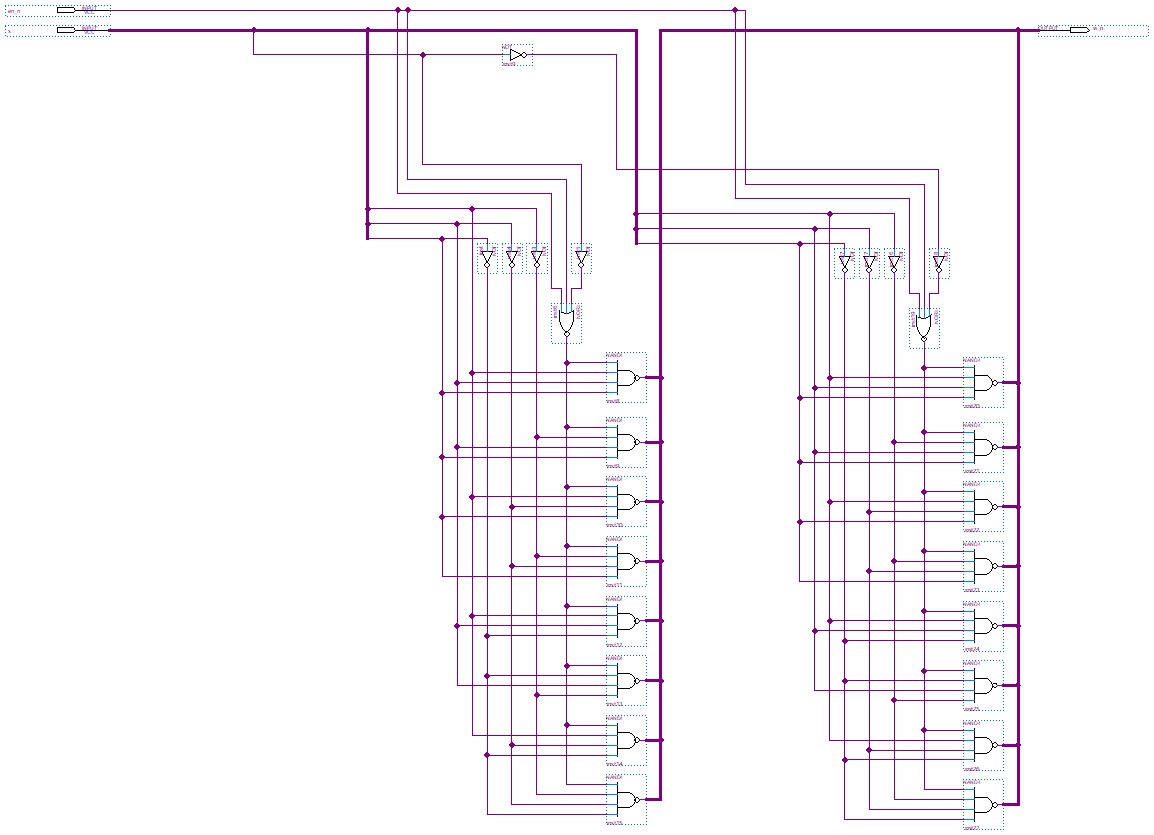
\includegraphics[width = .8\textwidth]{bdf2.png}}
\end{center}
These are both of the gate level diagrams of the two given circuits in the second diagram the two significant blobs of circuitry could have been replaced by a box representing the top circuit but I thought it would be more meaning full to see how easily using sub-modules can save the time to rewire and setup gates.
\section{Test Bench Comparisons}
The key difference between the two test bench files as far as I see is the choice to use a for loop to cut down the repetition in the code, since most of the lines in the first file were very similar bar one or two bits changing.

While both of these methods are effective at completing the task, when creating large test benches for bigger projects it would surely benefit you to use the for loops to test repetitive functions.
\section{Simulation Results}
\begin{center}
    \boxed{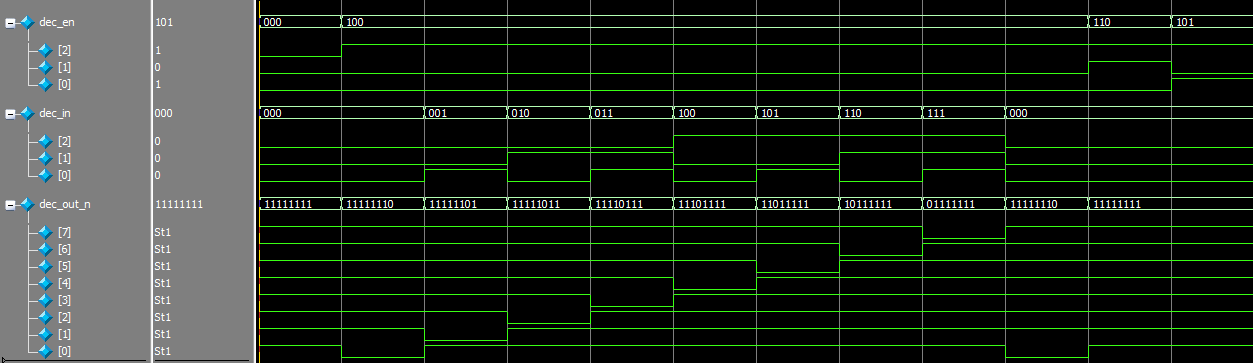
\includegraphics[width = .95\textwidth]{38decoder.png}}
    
    Above are the simulation results of the 3 to 8 decoder
\end{center}

\begin{center}
    \boxed{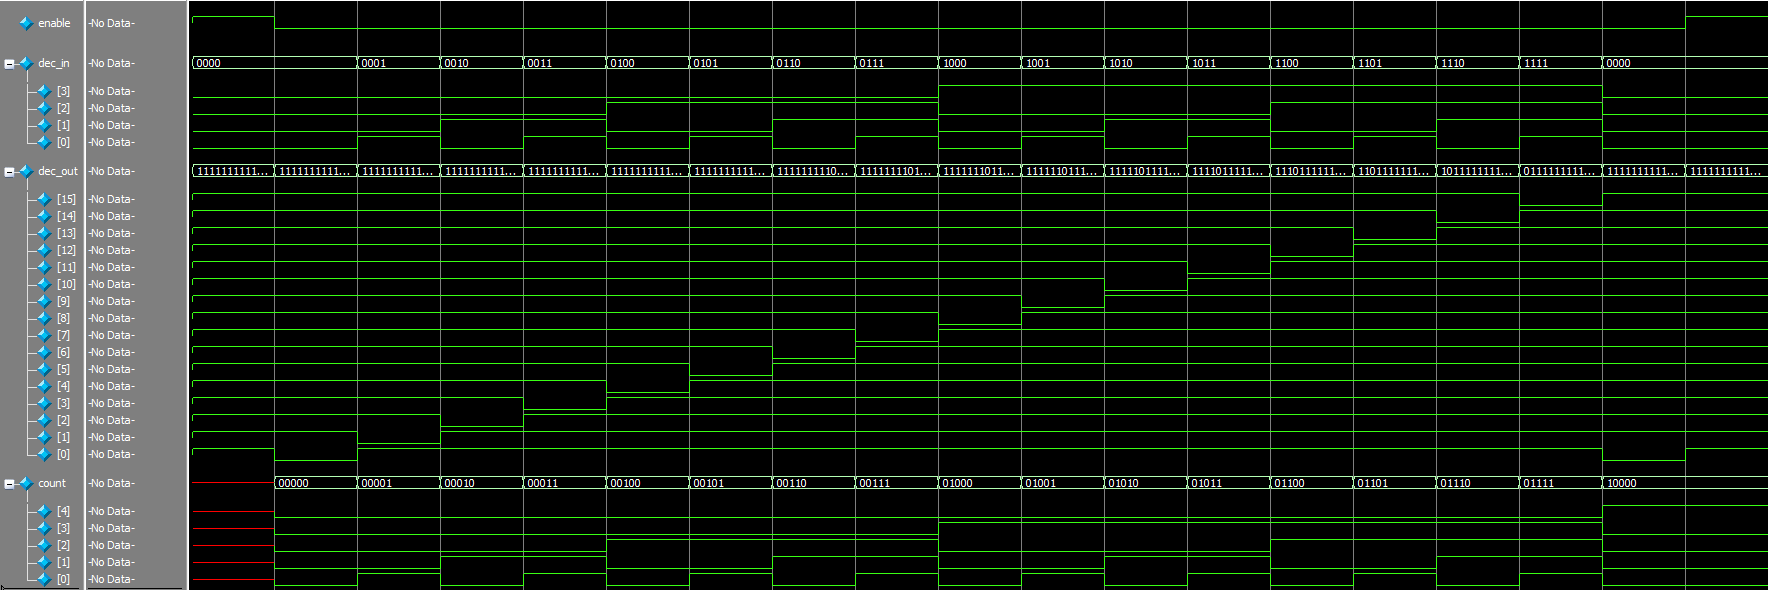
\includegraphics[width = .95\textwidth]{416decoder.png}}
    
    above are the simulation results of the 4 to 16 decoder
\end{center}
\section{RPS Design Approach}
The way I went about making this circuit and implementing it into Verilog was to first make a 6 variable truth table for all of the player inputs, then using the project specification, map each input set to an output, and anywhere there was an invalid player input I mapped all outputs to don't care conditions to save complexity (truth table seen below in section 6).

Once I did that I completed the 5 kmaps to find the simplest expression needed to get the correct output on each case. This allows me to save the most transistors compared to doing something like SOP which would be incredibly inefficient. I also only used NAND gates to save even more transistors compared to using AND and OR gates.

I do think that this is a viable design option in the real world because it tries to use the least amount of transistors, but it would be rather tedious to do this for every application so there may be an easier way to do it in the future.
\newpage
\section{RPS Truth Table}

\begin{center}
    \renewcommand{\arraystretch}{.95}
    \begin{tabular}{c|c|c|c|c|c|c|c|c|c|c}
        a[1] & a[0] & b[1] & b[0] & c[1] & c[0] & P1 & P2 &  P3 & TIE & REMATCH \\
        \hline
        0  &  0  &  0  &  0  &  0  &  0  &  0  &  0  &  0  &  1  &  0 \\
        0  &  0  &  0  &  0  &  0  &  1  &  X  &  X  &  X  &  X  &  X \\
        0  &  0  &  0  &  0  &  1  &  0  &  0  &  0  &  0  &  0  &  1 \\
        0  &  0  &  0  &  0  &  1  &  1  &  0  &  0  &  1  &  0  &  0 \\
        0  &  0  &  0  &  1  &  0  &  0  &  X  &  X  &  X  &  X  &  X \\
        0  &  0  &  0  &  1  &  0  &  1  &  X  &  X  &  X  &  X  &  X \\
        0  &  0  &  0  &  1  &  1  &  0  &  X  &  X  &  X  &  X  &  X \\
        0  &  0  &  0  &  1  &  1  &  1  &  X  &  X  &  X  &  X  &  X \\
        0  &  0  &  1  &  0  &  0  &  0  &  0  &  0  &  0  &  0  &  1 \\
        0  &  0  &  1  &  0  &  0  &  1  &  X  &  X  &  X  &  X  &  X \\
        0  &  0  &  1  &  0  &  1  &  0  &  0  &  0  &  0  &  0  &  1 \\
        0  &  0  &  1  &  0  &  1  &  1  &  0  &  0  &  0  &  0  &  1 \\
        0  &  0  &  1  &  1  &  0  &  0  &  0  &  1  &  0  &  0  &  0 \\
        0  &  0  &  1  &  1  &  0  &  1  &  X  &  X  &  X  &  X  &  X \\
        0  &  0  &  1  &  1  &  1  &  0  &  0  &  0  &  0  &  0  &  1 \\
        0  &  0  &  1  &  1  &  1  &  1  &  1  &  0  &  0  &  0  &  0 \\
        0  &  1  &  0  &  0  &  0  &  0  &  X  &  X  &  X  &  X  &  X \\
        0  &  1  &  0  &  0  &  0  &  1  &  X  &  X  &  X  &  X  &  X \\
        0  &  1  &  0  &  0  &  1  &  0  &  X  &  X  &  X  &  X  &  X \\
        0  &  1  &  0  &  0  &  1  &  1  &  X  &  X  &  X  &  X  &  X \\
        0  &  1  &  0  &  1  &  0  &  0  &  X  &  X  &  X  &  X  &  X \\
        0  &  1  &  0  &  1  &  0  &  1  &  X  &  X  &  X  &  X  &  X \\
        0  &  1  &  0  &  1  &  1  &  0  &  X  &  X  &  X  &  X  &  X \\
        0  &  1  &  0  &  1  &  1  &  1  &  X  &  X  &  X  &  X  &  X \\
        0  &  1  &  1  &  0  &  0  &  0  &  X  &  X  &  X  &  X  &  X \\
        0  &  1  &  1  &  0  &  0  &  1  &  X  &  X  &  X  &  X  &  X \\
        0  &  1  &  1  &  0  &  1  &  0  &  X  &  X  &  X  &  X  &  X \\
        0  &  1  &  1  &  0  &  1  &  1  &  X  &  X  &  X  &  X  &  X \\
        0  &  1  &  1  &  1  &  0  &  0  &  X  &  X  &  X  &  X  &  X \\
        0  &  1  &  1  &  1  &  0  &  1  &  X  &  X  &  X  &  X  &  X \\
        0  &  1  &  1  &  1  &  1  &  0  &  X  &  X  &  X  &  X  &  X \\
        0  &  1  &  1  &  1  &  1  &  1  &  X  &  X  &  X  &  X  &  X \\
        1  &  0  &  0  &  0  &  0  &  0  &  1  &  0  &  0  &  0  &  0 \\
        1  &  0  &  0  &  0  &  0  &  1  &  X  &  X  &  X  &  X  &  X \\
        1  &  0  &  0  &  0  &  1  &  0  &  0  &  1  &  0  &  0  &  0 \\
        1  &  0  &  0  &  0  &  1  &  1  &  0  &  0  &  0  &  0  &  1 \\
        1  &  0  &  0  &  1  &  0  &  0  &  X  &  X  &  X  &  X  &  X \\
        1  &  0  &  0  &  1  &  0  &  1  &  X  &  X  &  X  &  X  &  X \\
        1  &  0  &  0  &  1  &  1  &  0  &  X  &  X  &  X  &  X  &  X \\
        1  &  0  &  0  &  1  &  1  &  1  &  X  &  X  &  X  &  X  &  X \\
        1  &  0  &  1  &  0  &  0  &  0  &  0  &  0  &  1  &  0  &  0 \\
        1  &  0  &  1  &  0  &  0  &  1  &  X  &  X  &  X  &  X  &  X \\
        1  &  0  &  1  &  0  &  1  &  0  &  0  &  0  &  0  &  1  &  0 \\
        1  &  0  &  1  &  0  &  1  &  1  &  0  &  0  &  0  &  0  &  1 \\
        1  &  0  &  1  &  1  &  0  &  0  &  0  &  0  &  0  &  0  &  1 \\
        1  &  0  &  1  &  1  &  0  &  1  &  X  &  X  &  X  &  X  &  X \\
        1  &  0  &  1  &  1  &  1  &  0  &  0  &  0  &  0  &  0  &  1 \\
        1  &  0  &  1  &  1  &  1  &  1  &  0  &  0  &  0  &  0  &  1 \\
        1  &  1  &  0  &  0  &  0  &  0  &  0  &  0  &  0  &  0  &  1 \\
        1  &  1  &  0  &  0  &  0  &  1  &  X  &  X  &  X  &  X  &  X \\
        1  &  1  &  0  &  0  &  1  &  0  &  0  &  0  &  0  &  0  &  1 \\
        1  &  1  &  0  &  0  &  1  &  1  &  0  &  0  &  0  &  0  &  1 \\
        1  &  1  &  0  &  1  &  0  &  0  &  X  &  X  &  X  &  X  &  X \\
        1  &  1  &  0  &  1  &  0  &  1  &  X  &  X  &  X  &  X  &  X \\
        1  &  1  &  0  &  1  &  1  &  0  &  X  &  X  &  X  &  X  &  X \\
        1  &  1  &  0  &  1  &  1  &  1  &  X  &  X  &  X  &  X  &  X \\
        1  &  1  &  1  &  0  &  0  &  0  &  0  &  0  &  0  &  0  &  1 \\
        1  &  1  &  1  &  0  &  0  &  1  &  X  &  X  &  X  &  X  &  X \\
        1  &  1  &  1  &  0  &  1  &  0  &  1  &  0  &  0  &  0  &  0 \\
        1  &  1  &  1  &  0  &  1  &  1  &  0  &  1  &  0  &  0  &  0 \\
        1  &  1  &  1  &  1  &  0  &  0  &  0  &  0  &  0  &  0  &  1 \\
        1  &  1  &  1  &  1  &  0  &  1  &  X  &  X  &  X  &  X  &  X \\
        1  &  1  &  1  &  1  &  1  &  0  &  0  &  0  &  1  &  0  &  0 \\
        1  &  1  &  1  &  1  &  1  &  1  &  0  &  0  &  0  &  1  &  0    
    \end{tabular}
\end{center}
\section{RPS Structural Verilog Code}
\begin{center}
    \boxed{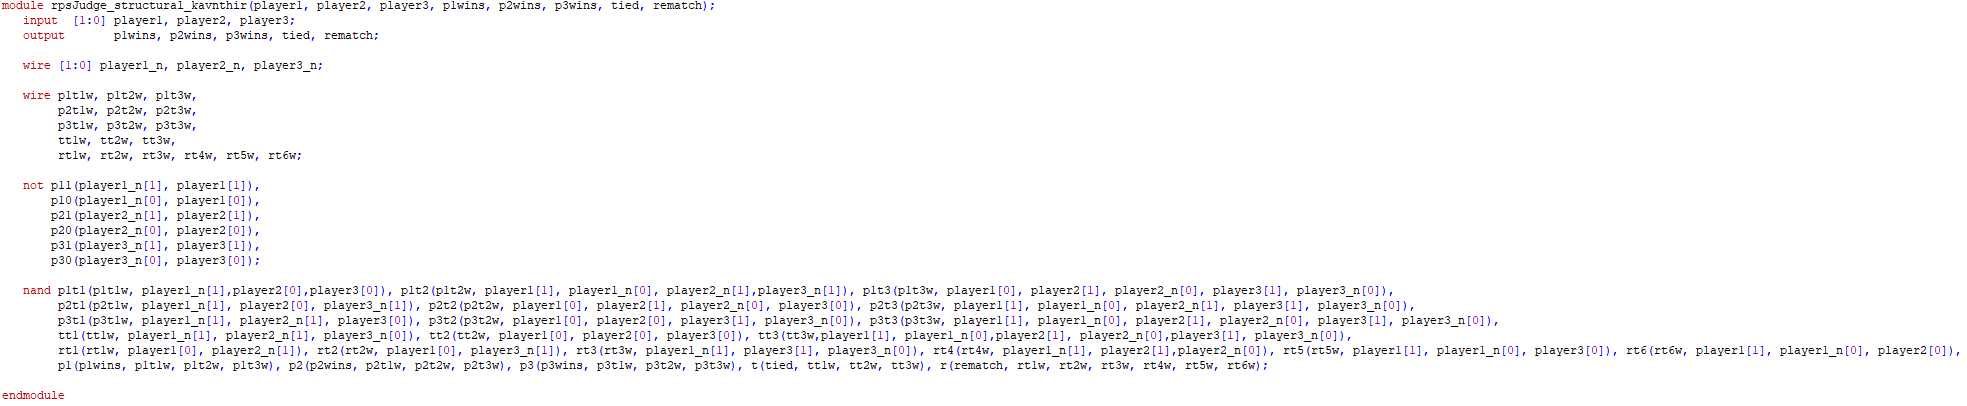
\includegraphics[width = .98\textwidth]{code.png}}
\end{center}
\section{RPS Structural Test Bench}
\begin{center}
    \boxed{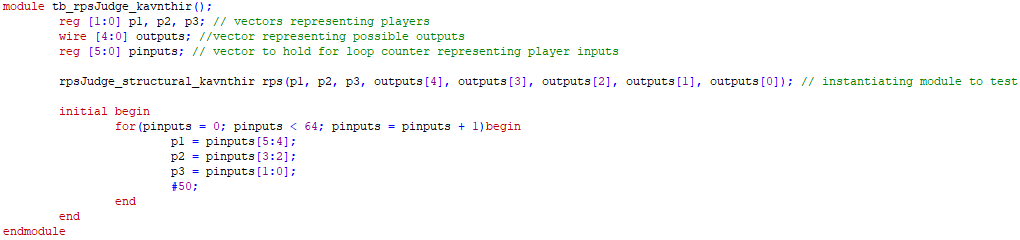
\includegraphics[width = .98\textwidth]{tb.png}}
\end{center}

The way I approached the test bench was to feed the inputs with every possible set of them, and I could cross reference the waveform with the truth table to see if the output is correct or not.

This approach is what was being using in 2544 to test so I assume it isnt the worst way to go about doing it. But at the same time I am not certain it is the best way but with the knowledge I currently have i'm not sure what would be the best way.

\section{RPS Simulation}

\begin{center}
    \boxed{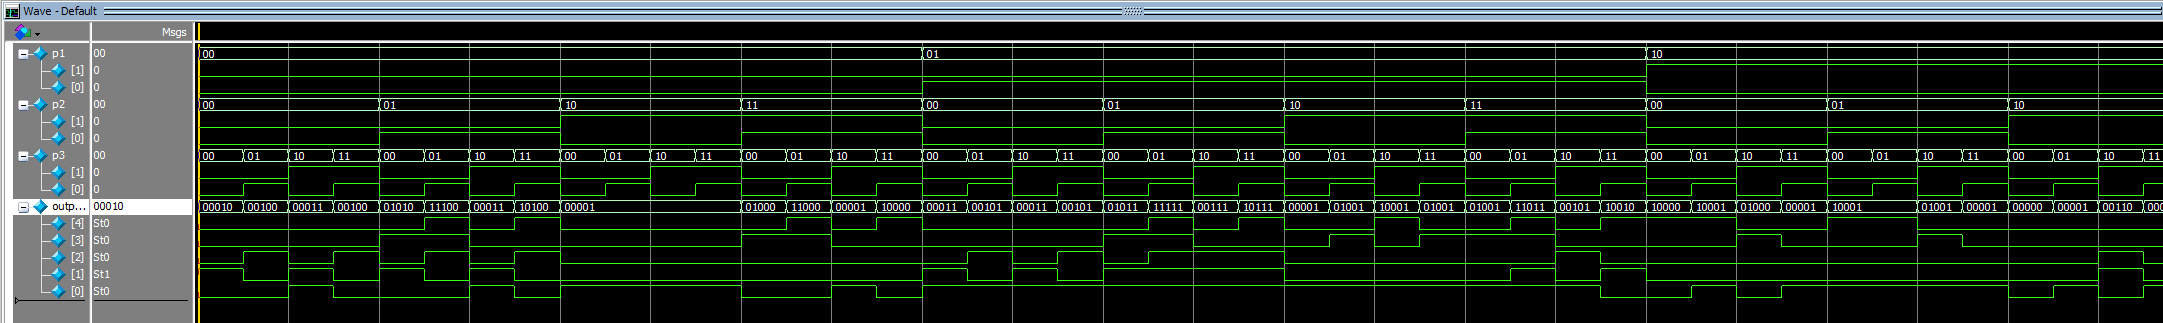
\includegraphics[width = .98\textwidth]{sim.png}}
\end{center}

\section{Conclusion}

I learned in this assignment that even things as simple as a game of rps can cause extremely large tedious truth tables that need to be solved, and I assume the job of a digital designer isnt just tediously solving kmaps and truth tables so there must be a better way to go about solving a problem like this.

If I were to guess it would be to sacrifice transistor efficiency and instead use layers of abstraction to construct a solution that would be easier to design.

\end{document}
